%% Преамбула TeX-файла

% 1. Стиль и язык
\documentclass[utf8x]{G7-32} % Стиль (по умолчанию будет 14pt)
%\documentclass{book} % Стиль (по умолчанию будет 14pt)
\usepackage[T2A]{fontenc}
\usepackage[russian]{babel}

% Остальные стандартные настройки убраны в preamble.inc.tex.

\usepackage{pdflscape}
\usepackage{svg}
\usepackage{longtable}
\usepackage{pdflscape}
\usepackage{lscape}
\usepackage{cancel}
\usepackage{wrapfig}
\usepackage{booktabs}
% Настройки листингов.
% 8 Листинги

\usepackage{listings}

% Значения по умолчанию
\lstset{
  basicstyle= \footnotesize,
  breakatwhitespace=true,% разрыв строк только на whitespacce
  breaklines=true,       % переносить длинные строки
%   captionpos=b,          % подписи снизу -- вроде не надо
  inputencoding=koi8-r,
  numbers=left,          % нумерация слева
  numberstyle=\footnotesize,
  showspaces=false,      % показывать пробелы подчеркиваниями -- идиотизм 70-х годов
  showstringspaces=false,
  showtabs=false,        % и табы тоже
  stepnumber=1,
  tabsize=4,              % кому нужны табы по 8 символов?
  frame=single
}

% Стиль для псевдокода: строчки обычно короткие, поэтому размер шрифта побольше
\lstdefinestyle{pseudocode}{
  basicstyle=\small,
  keywordstyle=\color{black}\bfseries\underbar,
  language=Pseudocode,
  numberstyle=\footnotesize,
  commentstyle=\footnotesize\it
}

% Стиль для обычного кода: маленький шрифт
\lstdefinestyle{realcode}{
  basicstyle=\scriptsize,
  numberstyle=\footnotesize
}

% Стиль для коротких кусков обычного кода: средний шрифт
\lstdefinestyle{simplecode}{
  basicstyle=\footnotesize,
  numberstyle=\footnotesize
}

% Стиль для BNF
\lstdefinestyle{grammar}{
  basicstyle=\footnotesize,
  numberstyle=\footnotesize,
  stringstyle=\bfseries\ttfamily,
  language=BNF
}

% Определим свой язык для написания псевдокодов на основе Python
\lstdefinelanguage[]{Pseudocode}[]{Python}{
  morekeywords={each,empty,wait,do},% ключевые слова добавлять сюда
  morecomment=[s]{\{}{\}},% комменты {а-ля Pascal} смотрятся нагляднее
  literate=% а сюда добавлять операторы, которые хотите отображать как мат. символы
    {->}{\ensuremath{$\rightarrow$}~}2%
    {<-}{\ensuremath{$\leftarrow$}~}2%
    {:=}{\ensuremath{$\leftarrow$}~}2%
    {<--}{\ensuremath{$\Longleftarrow$}~}2%
}[keywords,comments]

% Свой язык для задания грамматик в BNF
\lstdefinelanguage[]{BNF}[]{}{
  morekeywords={},
  morecomment=[s]{@}{@},
  morestring=[b]",%
  literate=%
    {->}{\ensuremath{$\rightarrow$}~}2%
    {*}{\ensuremath{$^*$}~}2%
    {+}{\ensuremath{$^+$}~}2%
    {|}{\ensuremath{$|$}~}2%
}[keywords,comments,strings]

% Подписи к листингам на русском языке.
\renewcommand\lstlistingname{\cyr\CYRL\cyri\cyrs\cyrt\cyri\cyrn\cyrg}
\renewcommand\lstlistlistingname{\cyr\CYRL\cyri\cyrs\cyrt\cyri\cyrn\cyrg\cyri}

\sloppy

% Настройки стиля ГОСТ 7-32
% Для начала определяем, хотим мы или нет, чтобы рисунки и таблицы нумеровались в пределах раздела, или нам нужна сквозная нумерация.
\EqInChapter % формулы будут нумероваться в пределах раздела
\TableInChapter % таблицы будут нумероваться в пределах раздела
\PicInChapter % рисунки будут нумероваться в пределах раздела

% Добавляем гипертекстовое оглавление в PDF
\usepackage[
bookmarks=true, colorlinks=true, unicode=true,
urlcolor=black,linkcolor=black, anchorcolor=black,
citecolor=black, menucolor=black, filecolor=black,
]{hyperref}

% Изменение начертания шрифта --- после чего выглядит таймсоподобно.
% apt-get install scalable-cyrfonts-tex

\IfFileExists{cyrtimes.sty}
    {
        \usepackage{cyrtimespatched}
    }
    {
        % А если Times нету, то будет CM...
    }

\usepackage{graphicx}   % Пакет для включения рисунков

% С такими оно полями оно работает по-умолчанию:
% \RequirePackage[left=20mm,right=10mm,top=20mm,bottom=20mm,headsep=0pt]{geometry}
% Если вас тошнит от поля в 10мм --- увеличивайте до 20-ти, ну и про переплёт не забывайте:
\geometry{right=20mm}
\geometry{left=30mm}


% Пакет Tikz
\usepackage{tikz}
\usetikzlibrary{arrows,positioning,shadows}

% Произвольная нумерация списков.
\usepackage{enumerate}

% ячейки в несколько строчек
\usepackage{multirow}

% itemize внутри tabular
\usepackage{paralist,array}
\usepackage{longtable}
% Любимые команды
\newcommand{\Code}[1]{\textbf{#1}}

% Полезные макросы листингов.


\title{Course-work}
\author{}
 

\begin{document}


%Изменим нумерацию на более привычную...
%... и нарушим этим гост.

\renewcommand{\labelenumi}{\arabic{enumi})}
\renewcommand{\labelenumii}{\asbuk{enumii})}


\frontmatter % выключает нумерацию ВСЕГО; здесь начинаются ненумерованные главы: реферат, введение, глоссарий, сокращения и прочее.

% Команды \breakingbeforechapters и \nonbreakingbeforechapters
% управляют разрывом страницы перед главами.
% По-умолчанию страница разрывается.

% \nobreakingbeforechapters
% \breakingbeforechapters


\pagestyle{empty} % нумерация выкл.

\begin{center}
    \textup{\textbf{NATIONAL RESEARCH UNIVERSITY} \\ \textbf{HIGHER SCHOOL OF ECONOMICS}} \\[5mm]

     \textup{Faculty of Computer Science  \\ Bachelor’s Programme “Data Science and Business Analytics”} \\[2mm]

 
       \textup{\large\bfseries
         \\[1mm] Research Project Report }\\[5mm] on the topic \\[5mm]
         \textbf{Long-Range Camera Guidance for Person Recognition in Public Spaces.}\\[5mm] 

\end{center}
\vspace{1mm}
\textbf{Fulfilled by the Student:}\\[2mm]

% \begin{tabular}{l@{\hskip 1cm}c@{\hskip 1cm}c}
% Student of the group \foreignlanguage{russian}{БПАД}212 & & \\
% Khaibrakhmanov Timur Radikovich & \rule{3.5cm}{0.15mm}  &  \rule{3.5cm}{0.15mm} \vspace{-2mm} \\
%  & \tiny{(signature)}  & \tiny{(date)} \\
% \end{tabular} \\


\begin{tabular}{l@{\hskip 0.7cm}c@{\hskip 1cm}c}
Student of the group \foreignlanguage{russian}{БПАД}213 & 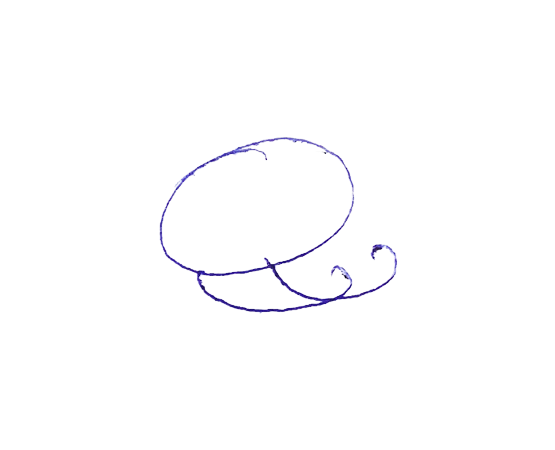
\includegraphics[width=0.12\linewidth]{Timchenko/sig.png}  & 02.06.2024\\
Timchenko Daniil Gennadievich & \rule{3.5cm}{0.15mm}  & 


\rule{3.5cm}{0.15mm} \vspace{-2mm} \\
 & \tiny{(signature)}  & \tiny{(date)} \\
\end{tabular}\\[3mm]
\textbf{Checked by the Project Supervisor:}\\[2mm]
\begin{tabular}{l@{\hskip 1.5cm}l}
Khelvas Alexander Valerievich\\
COO {JSC COS\&HT} \vspace{1mm}\\
% 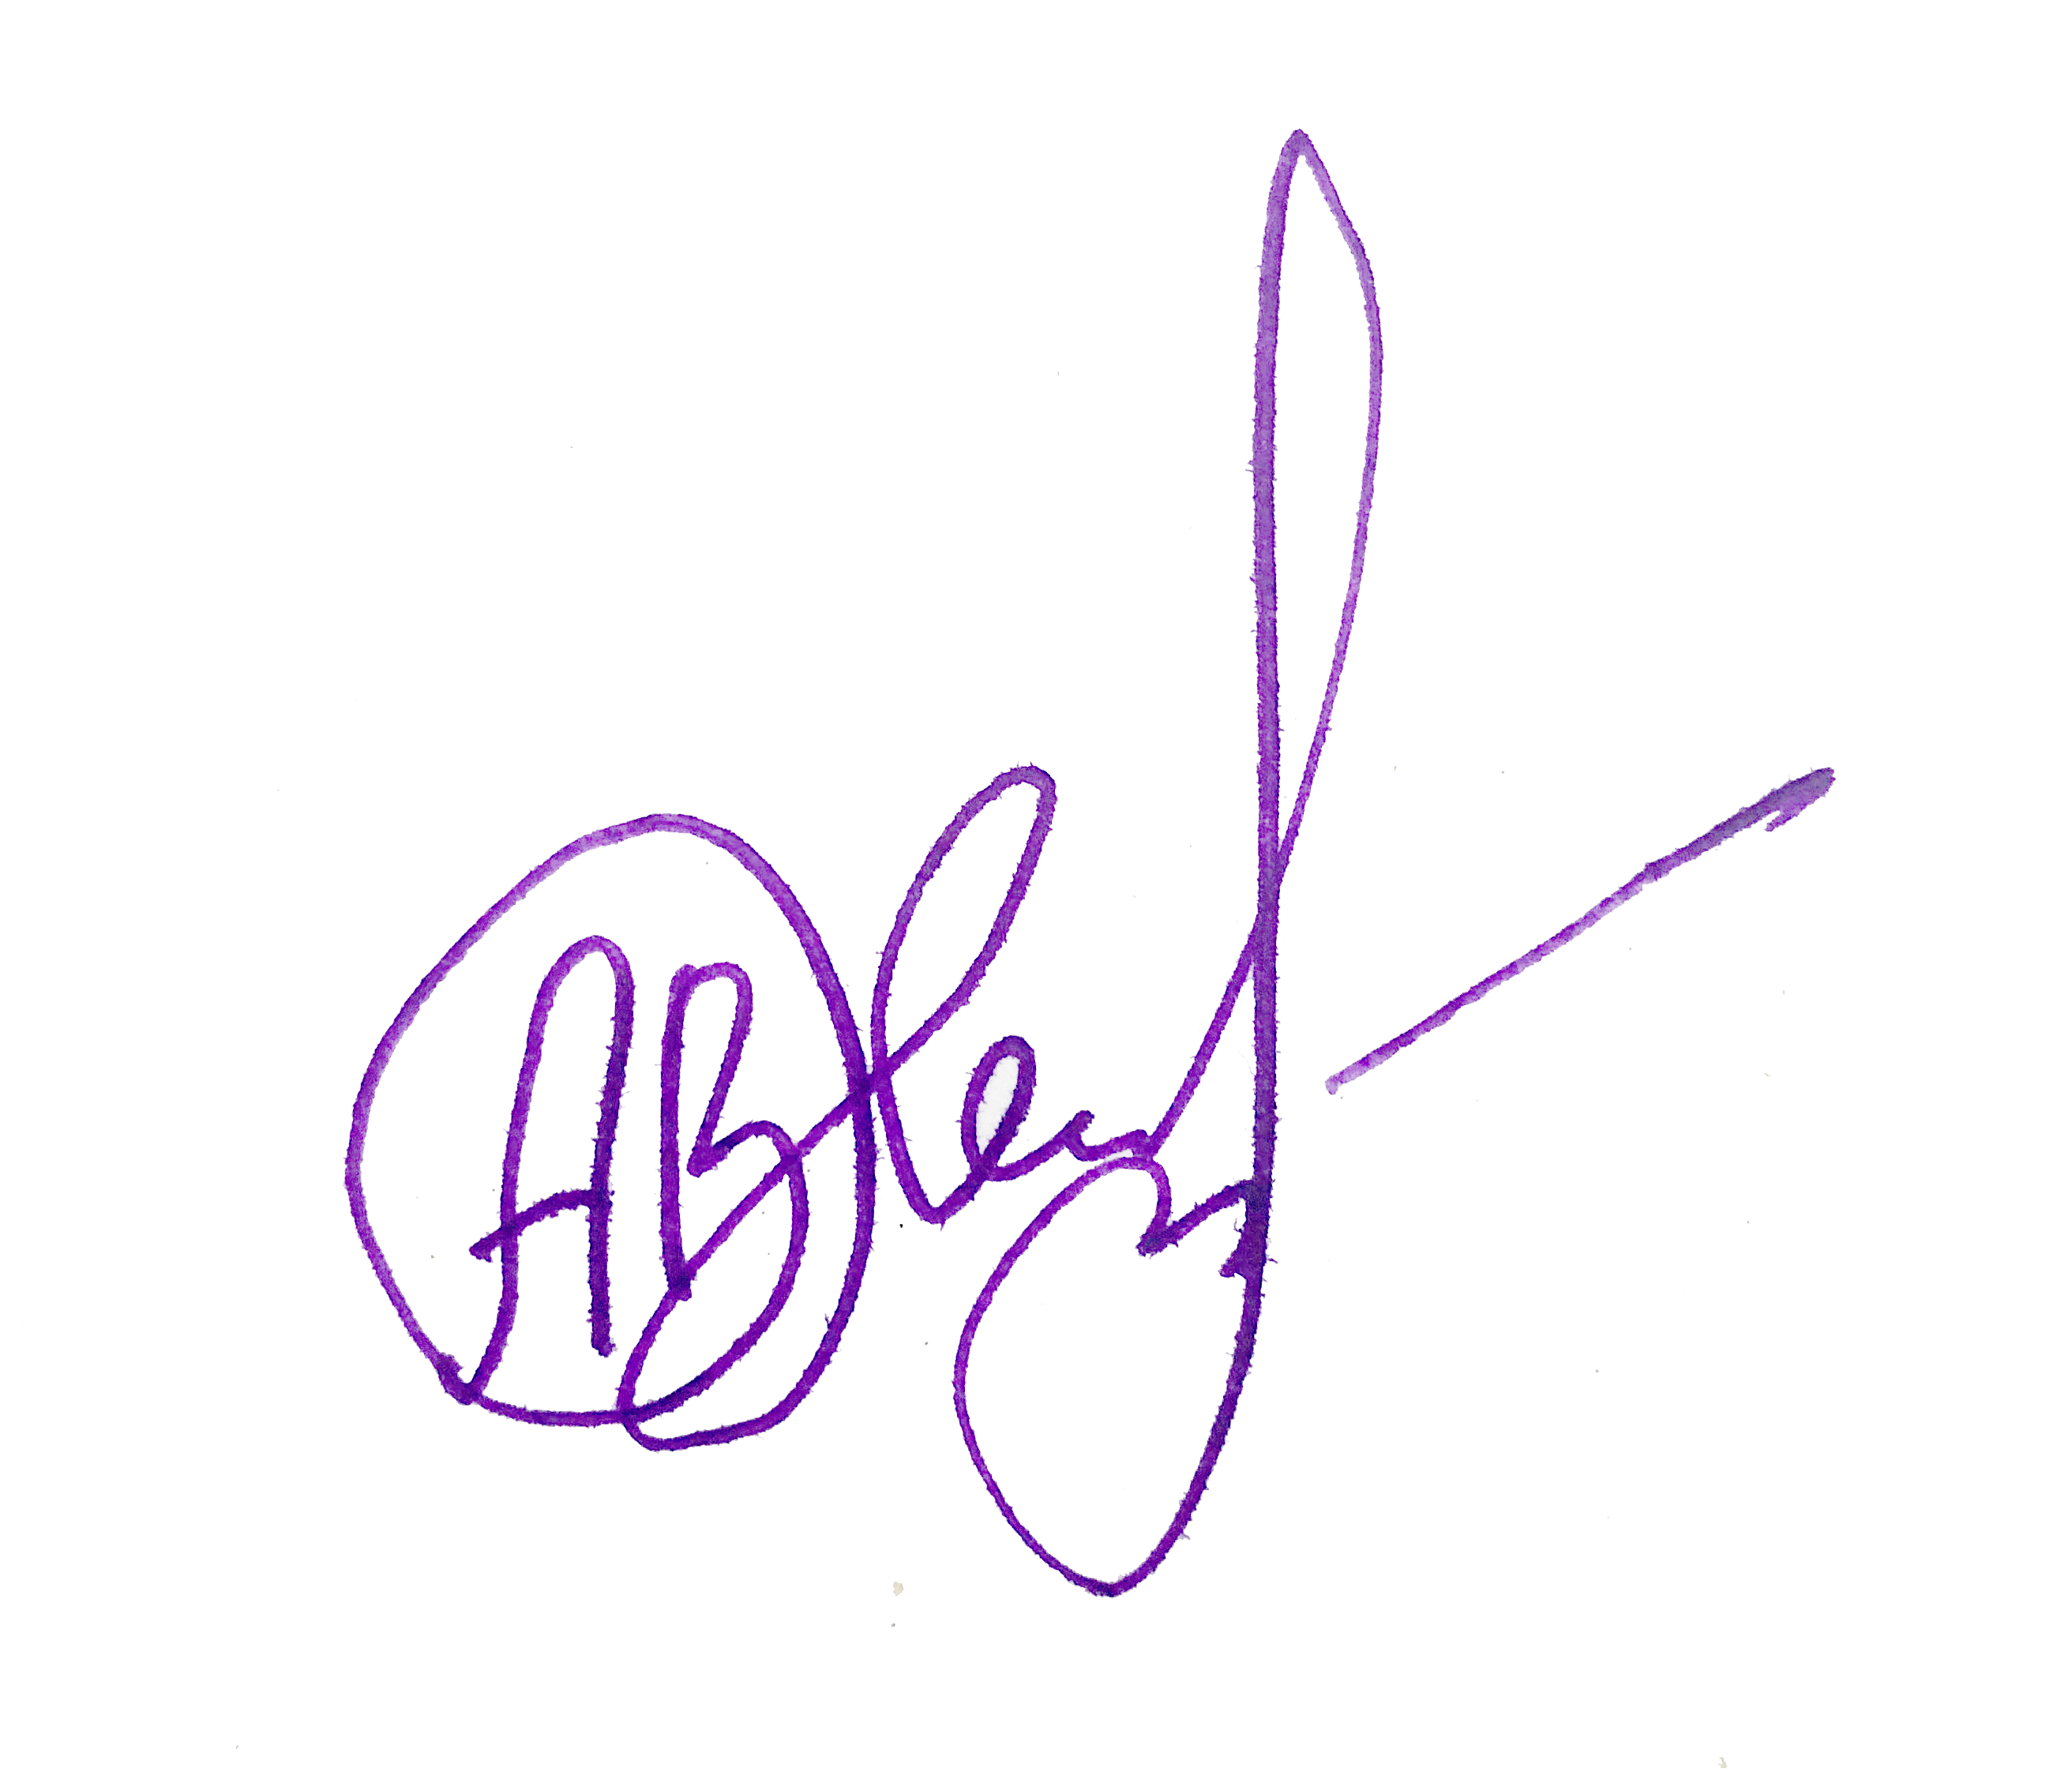
\includegraphics[width=0.32\linewidth]{figures/sign.png} \\ signature not needed from students
\rule{4cm}{0.15mm} 
 &\rule{4cm}{0.15mm} \vspace{-2mm}\\
{\hskip 1.5cm}\tiny{(signature)} & {\hskip 1.5cm}\tiny{(date)} \\
\end{tabular}


\vspace{\fill}

\begin{center}
Moscow 2024
\end{center}

%\end{titlepage}

% 

\newpage

\textbf{Список исполнителей}
\\[20mm]


  \begin{tabular}{p{150pt}p{100pt}p{100pt}} 
       Руководитель работы & &~ \\ [15pt]
       Исполнитель & &  \\ [25pt]
         & &~ \\ [15pt]

     
       
        
        
    \end{tabular}

\pagestyle{plain}  

% % Также можно использовать \Referat, как в оригинале
\begin{abstract}

{\color{red}Общие правила 

1) не используем принудительную разметку страниц 

2) картинки лежат в папках figures и eps (при этом все графики и схемы должны быть в eps)  Шрифт на картинках не должен быть меньше 12. Если на картинке используется текст - должны быть русский и английский варианты. 

3) Все публикации на которые ссылаемся должны быть в bibtex в bib файле

\color{blue} 4) Синим цветом помечены куски которые должны быть переизложены для антиплагиата. Это прямые заимствования}




Авторы  

Хайбрахманов Тимур Радикович (trkhaybrakhmanov@edu.hse.ru)

Тимченко Даниил Геннадьевич (dgtimchenko@edu.hse.ru)

Authors  

Khaibrakhmanov Timur Radikovich

Timchenko Daniil Gennadyevich



Объем отчета - 18 стр.%,  таблиц -1 , приложений - 1.

Ключевые слова:  Алгоритм управления длиннофокусной камерой, Задача коммивояжёра (Travelling Salesman Problem, TSP), Распознавание объектов.
 



\end{abstract}
\pagestyle{plain} % нумерация вкл.
 

\tableofcontents



% %\Defines % Необходимые определения. Вряд ли понадобться

% \chapter{Термины и определения}

% \vspace{20pt}

% \begin{description}

% \item [Искусственный интеллект (далее - ИИ)] - комплекс технологических решений, позволяющий имитировать когнитивные функции человека (включая самообучение и поиск решений без заранее заданного алгоритма) и получать при выполнении конкретных задач результаты, сопоставимые, как минимум, с результатами интеллектуальной деятельности человека. Комплекс технологических решений включает в себя информационно-коммуникационную инфраструктуру, программное обеспечение (в том числе в котором используются методы машинного обучения), процессы и сервисы по обработке данных и поиску решений;
%  \item [g43]
% \end{description}

 
% \Abbreviations %% Список обозначений и сокращений в тексте
% \begin{description}
% \item [ASR] automatic speech recognition (автомаическое распознавание речи)
% \item [CSV]  
%  (CSV от англ. Comma-Separated Values — значения, разделённые запятыми) — текстовый формат, предназначенный для представления табличных данных
% \item [Dynamic HTML]
% набор средств, которые позволяют создавать более интерактивные Web-страницы без увеличения загрузки сервера
% \item [HTML] 
% Язык гипертекстовой разметки документов (от англ. Hypertext Markup Language – “язык гипертекстовой разметки”)
% \item [HTTP] 
% Протокол прикладного уровня для передачи данных, используемый в Web (от англ. HyperText Transfer Protocol - «протокол передачи гипертекста») 
% \item [IP-адрес] 
% Уникальный сетевой адрес узла в компьютерной сети, построенной по протоколу IP
% \item [JavaScript]  Прототипно-ориентированный сценарный язык программирования. Наиболее широкое применение находит в браузерах как язык сценариев для придания интерактивности веб-страницам
% \item [JPEG (JPG)] JPEG - один из популярных графических форматов, применяемый для хранения фотоизображений и подобных им изображений. Файлы, содержащие данные JPEG, обычно имеют расширения .jpg, .jfif, .jpe или .jpeg.
% \item [MS SQL]  Microsoft SQL Server — система управления реляционными базами данных (РСУБД), разработанная корпорацией Microsoft
% \item [PDF]  Portable Document Format (PDF) — межплатформенный формат электронных документов, разработанный фирмой Adobe Systems
% \item [PHP] Cкриптовый язык общего назначения, интенсивно применяемый для разработки веб-приложений.
% \item [PNG]  Растровый формат хранения графической информации, использующий сжатие без потерь качества

% \item [НСИ] 
% Нормативно – справочная информация
% \item [НИР] Научно - исследовательская работа
% \item [АС]  Автоматизированная система
% \item [Интернет]  Информационно-телекоммуникационная сеть Интернет


% \item [Открытые данные] 
% Информация, размещаемая ее обладателями в сети «Интернет» в формате, допускающем автоматизированную обработку без предварительных изменений человеком в целях повторного ее использования

% \item [ПО]  
% Программное обеспечение
% \item[АИС] Автоматизированная информационная система. Но надо протестировать длинные строки в определениях.
% \item[АРМ] Автоматизированная рабочее место
% \item[КВиВ] Подсистема комплексного мониторинга компонент видеомониторинга и видеоанализа 
% \item[МВЯ] Модуль вычислительного ядра  
% \item[МВЯ] Модуль хранения видеоинформации (архив) 
% \item[CPU] Central processing unit 
% \end{description}

% %%% Local Variables:
% %%% mode: latex
% %%% TeX-master: "rpz"
% %%% End:



%\include{12-intro}


\mainmatter % это включает нумерацию глав и секций в документе ниже



% \include{1-Osnovania}  % Постановка задачи

% \chapter*{Research}

\paragraph{Objective of the research} - development of algorithms for controlling a long-focus camera observing many objects moving in two-dimensional or three-dimensional space.


\paragraph{Goals of the study} - 

\begin{itemize}
    \item Analysis of available scientific and patent literature on the topic and registration of patent search results.
    \item Preparation and marking of data used in the project.
    \item Modeling and its software implementation
    \item Analysis of results and preparation of publication based on the results of the work
\end{itemize}


\paragraph{Planned results} - 

\begin{itemize}
    \item Labeled data array.
    \item Software-implemented model.
    \item Scientific and technical report.
    \item Publication in "Computer Research and Modeling".
    
\end{itemize}

All code and data for project are available in \href{https://github.com/mikecarti/hse-cam2023}{https://github.com/mikecarti/hse-cam2023}

\chapter{Description of the problem setting for the course work}
\label{cha:Osnovania-ENG}

\section{Terminology}

\subsection{Focal Length}
Focal length is a distance between "nodal point" (that is where light converges in a lens) and a camera sensor\cite{FocalLength}. Cameras have a base focal length (max), but some cameras provide with a possibility to vary focal length by increasing/decreasing length of a camera lens. Thus a range of focal length ($F=(F_{min},F_{max})$) is of interest, as applications imply usages with long focus lenses.

 % \begin{figure}[!htbp]
 %     \centering
 %     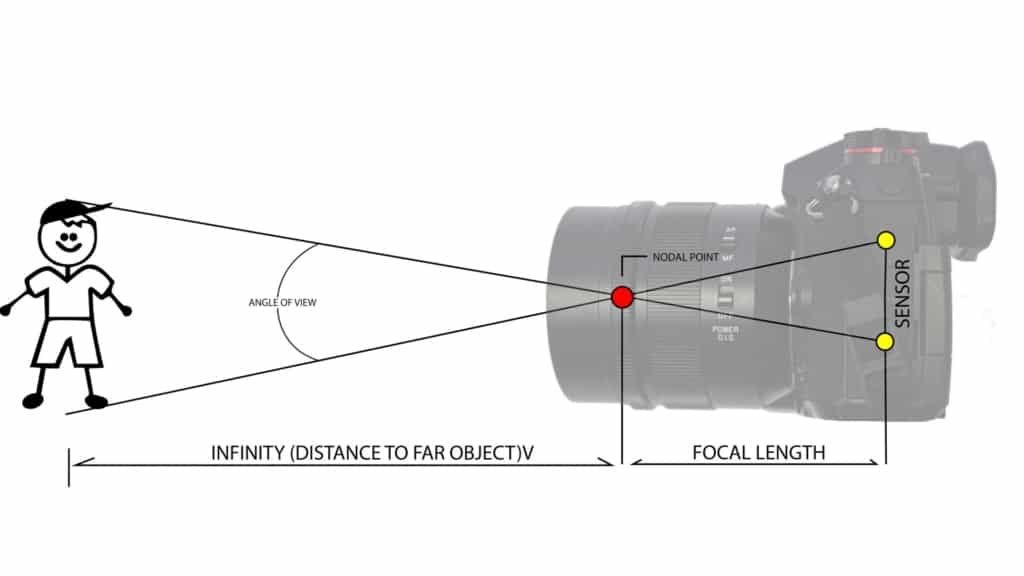
\includegraphics[width=0.8\linewidth]{figures/focal.jpg}
 %     \caption{Focal Length}
 %     \label{fig:enter-label}
 % \end{figure}

\subsection{Image sensor}
 An image sensor refers to the electronic component in a digital camera that captures and converts light into digital signals, ultimately creating a digital image. The image sensor plays a crucial role in digital photography by replacing the traditional film used in film cameras. $U=(u_1,u_2)$ - sensor size of a camera in pixels represents number of pixels along $x$ and $y$ axes respectively, total image might have upmost $u_1*u_2$ pixels, given that photo is RGB, it can be calculated, that on an 3-dimensional tensor with shape $(u_1, u_2, 3)$ the whole image can be stored, and on 4-dimensional tensor with shape $(u_1, u_2, 3, \textbf{frames})$ a whole video may be stored frome such camera without audio-stream, where frames - is the amount of frames taken from that camera consequently.



\subsection{Angular Velocity}
An angular velocity is the speed of rotation for an object that can be stated as ${\displaystyle \omega ={\frac {d\varphi }{dt}}}$.

\subsection{Elevation}
Vertical angle of an observed object over true horizon. Elevation combined with azimuth are used for obtaining the direction to an object. \href{https://ru.wikipedia.org/wiki/%D0%A3%D0%B3%D0%BE%D0%BB_%D0%BC%D0%B5%D1%81%D1%82%D0%B0}{Elevation}

\subsection{Azimuth}
Horizontal angle evaluated from predefined direction (for example north) and direction of an observed object.

\subsection{PTZ Camera}
is also known as pan-tilt-zoom camera is a type of cameras that is able to rotate across all 3 axis of rotation.

\section{Work Plan}

\begin{enumerate}
    \item Familiarize oneself with the literature.
    \item Formulate the goal and objectives of the work.
    \item Transition from a camera view to a top view (Projective Geometry).
    \item Solve the TSP problem for navigating players statically positioned on the field.
    \item Develop a simulation for debugging and testing the long-focus camera control algorithm.
    \begin{enumerate}
        \item Develop simulations of camera projection onto the field (3D).
        \item Develop an API to control the camera in the simulation.
        \item Integrate object behavior simulation with camera simulation.
    \end{enumerate}
    \item Develop a metric that fairly evaluates the algorithm's performance.
    \item Develop a camera control algorithm with the best metrics.
    \begin{enumerate}
        \item Implement field traversal through points most visited by each player without predicting player movement (find the most frequent point for each player).
        % \item Represent camera movement as a superposition of camera movement between zones and in a reference system tied to each zone.
        \item Implement player traversal considering predictions of player movement.
    \end{enumerate}
    \item Implement a PTZ camera model considering speed and acceleration constraints imposed on it. In the simplest case, neglect oscillations.
    \item Summarize the results.
\end{enumerate}

\section{Assumptions}

1. The input data is well-labeled and accurately reflects the true locations of objects, with IDs not getting mixed up.

2. One camera has a view of the entire field, while the other is a telephoto camera.

3. If a face is turned within ±45 degrees towards the camera, it is considered possible to photograph (so positions of players are known at a given moment).

4. The height of the players is 170 cm, with the possibility of setting individual values.

5. If the face is captured within 150 pixels under the condition of point 3 and is not obstructed by other players, the player is photographed.

\section{Problem Statement}

Develop a mechanism for controlling a long-focus camera for efficient player detection and tracking within the field of view. A cyclic process is proposed, within which the camera automatically switches between players, adjusting the viewing angle and shooting distance. At the beginning of each iteration, the camera is focused on a new player, and the distance between them and the camera is optimized until the player's silhouette or face occupies a specified percentage of screen space - n\% (with a tolerance). After that, the camera remains fixed on the player for a certain number of frames k before moving to the next player for the next iteration of the process.

When using the term 'efficiently' in this context, it implies that the algorithm should perform optimally on various datasets, such as video recordings of football matches with player labels and their positions in each frame. An algorithm tested on a subset taken from the population of football matches should perform traversal with shooting in the shortest time possible.

\subsection{Coordinate Transformation}
A projectivity from one projective plane to another is called a plane-to-plane projectivity, though it is often simply referred to as a projectivity. It operates on and produces a homogeneous 3-vector, thus represented as a 3-by-3 matrix.

To understand how such a projectivity occurs, consider two images taken from different viewpoints of a plane within a scene, as illustrated in Figure 1. The mapping of points to their corresponding points in image 1 is defined by a projectivity. Similarly, the mapping of points to their corresponding points in image 2 is defined by another projectivity. An essential characteristic of projectivities is that they form a group. Consequently, there exists a projectivity that describes the mapping from the image of the plane in image 1 to the image of the plane in image 2 where.
$$ R = ST^{-1}$$

Given particular coordinates $X,\;Y$ a plane-to-plane projective transformation can be done as following:

$$
\begin{bmatrix}
\tau_{i}X' \\
\tau_{i}Y' \\
\tau_{i}
\end{bmatrix} = 
\underbrace{ \begin{bmatrix}
a_{1} & a_{2} & b_{1} \\
a_{3} & a_{4} & b_{2} \\
c_{1} & c_{2} & 1
\end{bmatrix} }_{ M } \begin{bmatrix}
X \\
Y \\
1
\end{bmatrix}
$$

Where $a_i$ are elements of a scaling/rotation matrix, $\begin{bmatrix}
    b_2 & b_1
\end{bmatrix}^T$ is a translation vector and $\begin{bmatrix}
    c_1 & c_2
\end{bmatrix}$ is a projection vector.

To find true new coordinates $X', Y'$ resulting vector has to be divided by $\tau_i$ that is the scaling factor. 

\subsubsection{Code implementation}

Given source image field corner coordinates in a list corner\_src\_points, a projective transformation matrix can be calculated. Function cv2.getPerspectiveTransform takes 2 arguments: source (4 coordinates (x,y), resembling corners of the input quadrilateral) and destination (4 coordinates (x,y), resembling corners of the output quadrilateral). On output the projective transformation matrix $M \in \mathbb{R}^{3 \times 3}$ described above is obtained.

\lstinputlisting[language=Python]{listings/projective_matrix.py}

\pagebreak

\lstinputlisting[language=Python]{listings/coordinates_trans.py}
% add a link to library
Now by using this function and warpPerspective function from \textcolor{purple}{opencv} library, transformation can be done:
\begin{lstlisting}
corrected_image = cv2.warpPerspective(image, M, (width, height), borderValue=(255,255,255))
transform_coordinates(file_name="unscaled_track_df_new_coords.csv")
\end{lstlisting}

\section{Structure of the data}

Given a football field on which there are players and a ball, specified by coordinates $\vec X$, as functions of time $t$, in the reference system associated with the field. So we have an input array $X^{nm}_i$, where

$n$ - player number;

$m$ - describes one of the coordinates of the player’s position;

$i$ - describes a moment in time.

It is necessary to build a high-resolution camera axis control function (reserve $k$ for the camera number) with the given characteristics:

$F=(F_{min},F_{max})$ - focal length range;

$U=(u_1,u_2)$ - camera matrix size in pixels;

$p$ - matrix pixel size in meters (real world size of an image sensor's pixel);

$\Omega=(\omega_1, \omega_2)$ - maximum angular velocity in elevation and azimuth;

$\frac{dF}{dt}_{max}$ - maximum rate of change of focal length over time.

Camera coordinates in the reference system associated with the far left corner of the field

$$W=\{w_1,w_2,w_3\}$$




\section{The simplest task of controlling a high-resolution camera}

It is necessary to propose an algorithm for bypassing all players on the field, starting from the center of the field.

As a result we should get:

$\vec \psi(t)$ is a vector describing the elevation angle and azimuth of the camera sighting as a function of time.

At the same time, we must ensure that the player’s image is obtained in the camera’s field of view during the time $\Delta T$ corresponding to $R$ frames.

We consider the movement of the players to be a prior unknown.

1) The first step is to bypass stationary players

2) Second step - bypassing moving players

% Timur's part
% \subsection{Bypassing stationary players}

% Given a weighted graph $G = (V, E)$, in our case complete, since from any vertex it can be rational to move to another, in the general case, where

% $V$ - number of objects recognized in the frame, at this stage football players, $V = {1, 2, 3, ..., k}$

% $E$ - edges of this graph;

% $d_{ij}(i, j \in V, i \neq j)$ - the distance between two vertices $i, j$, and $d_{ij} > 0$, $d_{ij} \neq \infty$ and $d_{ij} = d_{ji}$.

% We need to find a Hamiltonian cycle (closed path) such that
% \begin{align}
%      minD = \sum_{i,j \in V} d_{ij} * x_{ij},
% \end{align}
% Where
% \begin{equation}
%      x_{ij} =
%      \begin{cases}
%          1 & e_{ij} \in \text{optimal path}\\
%          0 & e_{ij} \notin \text{optimal path}
%      \end{cases}
% \end{equation}
% That is, $x_{ij}$ is a logical variable that turns to 1 if the edge $e_{ij}$ satisfies the condition of belonging to the optimal path, and 0 otherwise. The start and end of the round generally take place in the center of the football field. The result of the algorithm should be a path containing all the vertices of the graph and satisfying the conditions specified above.

\section{Approximations and limitations}
 
Moving the camera angle up/down left/right and focusing are independent of each other and can be done in parallel. (The metric being optimized depends on this). We plan to have a different number of facilities and much greater than the number of football players. (The choice of algorithm depends on this - since the problem is NP hard, for a small amount it can be solved head-on - the 22 hypothesis is more optimal). The camera should return to the starting point (center by default).

 
% It is impossible to assume that the running speed of a football player is negligible relative to the speed of the camera.


\chapter{Formal problem statement}
\label{cha:Proposal-ENG}
  
 \section{The problem of traversing a set of moving points on a surface}

% {\color{red} Обращаю внимание что это не совсем задача описанная в статье - тут ребра графа меняются взаимосвязанным образом и корректно говорить все таки о задаче в ее первозданном виде. Необходимо тут сформулировать задачу в терминах поиска пути на графе заданного множеством вершин $A$ с длиной ребер вычисляемой, как функция времени.}

\iffalse % comment out large portion
Let us start from afar.  Assume that there exist a set of points $a=(x,y) \in\mathcal{A}$ on 2-dimensional surface, all these points coexist with some coordinates that describe their positions. 
These points coexist in an (assumably) discrete time interval 
$T$ ($T=\{1,2,3,\dots,k,\dots,t \}$). 
Assume all these points have their vectors, which represent their positions during every time index $i$. 

$$
\alpha_{j} = \begin{bmatrix}
a_{0} \\
a_{1} \\
\vdots \\
a_{k} \\
\vdots \\
a_{t}
\end{bmatrix} = \begin{bmatrix}
x_{0}  & y_{0} \\
x_{1}  & y_{1} \\
\vdots & \vdots\\
x_{k}  & y_{k} \\
\vdots & \vdots\\
x_{t}  & y_{t}
\end{bmatrix} \quad \forall \alpha_j \in \mathcal{A}
$$

On each time step $i$ it is trivial to show, that such set of points may be converted in a fully connected graph $G$, where nodes represent points $a$ and vertices represent the euclidean distance between two points. Then the optimization goal would be as follows: Given history of movement $T_{[1,k]} = \{1,2,...,k\}$ for $a_j \in \mathcal{A}$ find such path that it would be the fastest given the fact, that traveling speed $V$ is fixed (assumption), given the fact that movement for the period $T_{[k+1, t]}$ is unknown.

To simplify this, let us assume, that we already have a *good enough* predicting algorithm to know not only $T_{[1,k]}$ but $T_{[k+1, t]}$ as well. Then the formal statement from 1.4.1 is a modified:
... To be continued.

\fi % end of commenting out large portion

The problem of fast traversal of dynamic systems is a critical problem in the context of surveillance, safety, logistics and other fields. In our concrete case, we aim to develop an algorithm, able to traverse with long-focus camera those dynamic agents in the shortest time possible (or close to it). Advancements in this research could help across different fields, such as human surveillance, sport stadiums, city safety and etc. Thus provided with the purpose let us dive into the formal statement of a problem. 

Let $\mathbb{R}^{3}$ be the vector space, and $P_{t}$ = $\{ (x_{1}^{(t)},y_{1}^{(t)}), \dots, (x_{n}^{(t)},y_{n}^{(t)}) \}$ would be a set of observed objects existing in this vector space, that lie on a plane $z=0$ in moment of time $t \, \in \, \mathbb{N}$ ($x,y \, \in \, \mathbb{R}$). Let $\mathcal{P}$
$$\mathcal{P}_{t}(\hat{x}, \hat{y}, \hat{z}, \phi_{t}, \psi_{t}, \theta_{t},) \to \mathcal{V}$$
be the projection function that calculates corner points of FOV projection $\mathcal{V}_{t}$ $\, \in \, \mathbb{R}^{{3\times4}}$ on $z=0$ in the moment $t$. Here $\hat{x}, \hat{y}, \hat{z}$ - coordinates of a camera, $\phi_{t}, \psi_{t}, \theta_{t}$ - yaw (azimuth), pitch (elevation)  and roll in the time moment $t$ (rotation coordinates).
%% and $\zeta$ - is the zoom factor.  %%

Let $\mathcal{C}$
$$
\mathcal{C}(P_{t}, \mathcal{V}_{t}) \to \begin{bmatrix}
\Delta\phi_{t}  &  \Delta\psi_{t}  &  \Delta\theta_{t} 
\end{bmatrix}^{T}
$$
be the controller function, that makes a decision on the controlling of camera direction and zoom for the time-step $t+1$.  Camera rotations then are updated as following:
$$
\begin{bmatrix}
\phi_{t+1}   \\
 \psi_{t+1} \\
  \theta_{t+1} 
\end{bmatrix} = 
\begin{bmatrix}
\phi_{t}   \\
 \psi_{t} \\
  \theta_{t}
\end{bmatrix} + 
\begin{bmatrix}
\Delta\phi_{t}  \\
 \Delta\psi_{t}  \\
 \Delta\theta _{t}
\end{bmatrix}
$$

Let $\mathcal{I}$ 
$$
\mathcal{I}_{t}(\mathcal{P_{t}}, \mathcal{V}_{t}, p_{1}, p_{2}) \to a \, \in \, \{ 0,1 \}
$$
Be the indicator function, concluding if an observed object is taking up from $p_{1}$ to $p_{2}$ portion of space on a viewfinder AND never was observed in proper ratio before ($p_{1} \leq p \leq p2$). $a$ in this case is an indicator (True or False).

Then the constrained optimization problem looks as following:
$$
\begin{cases}
\sum\limits_{t=1}^{T} \mathcal{I}_{t}(\mathcal{P_{t}}, \mathcal{V}_{t}, p_{1}, p_{2}) \geq n \\
T \to \min\limits_{\mathcal{C}}
\end{cases}
$$



\section{An alternative formulation of DTSP in the general case}
DTSP is defined on a complete bidirectional graph $ G = (V, E) $, where $ V $ is the set of vertices of size $ n $ and $ E $ is the set of edges. $ V $ consists of a depot 0 and a set of potential agents. We consider an asymmetric distance in DTSP. Thus, $ E $ includes edges in both directions. The agents to be visited are placed in a pool of agents $ C $ of size $ c $, where $ C $ is a subset of $ V $.

The salesman starts his journey from depot 0 at the beginning of time (t = 0). He must service each agent in the pool $ C $ exactly once and then return to the depot. The travel time from vertex $ i $ to vertex $ j $ depends on a time-dependent function $ g_{ij} (t) $, where $ t $ is the time to visit vertex $ i $. We assume that the seller does not wait at a vertex. This is true when the FIFO (First-In-First-Out) constraint is satisfied, i.e., it is guaranteed that if a vehicle leaves vertex $ i $ for vertex $ j $ at a certain time, any identical vehicle leaving vertex $ i $ for vertex $ j $ at a later time will arrive later at vertex $ j $.

Let $ x_{ij} $ be a binary decision variable that equals 1 if the seller travels from vertex $ i $ to vertex $ j $, and 0 otherwise.

Let $ s_i $ be the time when the seller visits vertex $ i $. The objective is to minimise the total travel time to visit all agents, i.e.

$$
\min_{}\sum_{i\, \in\, \{ 0 \}\cup C}\;\sum_{j\, \in\, \{ 0 \}\cup C} g_{ij}(s_{i})x_{ij}
$$

Set of constraints:


\begin{align}
\sum_{j \, \in \, \{ 0 \}\cup C} x_{ij} = 1 \quad  \forall i \, \in \, C \\
\sum_{i \, \in \, \{ 0 \}\cup C} x_{ji} =1 \quad  \forall i \, \in \, C \\
s_{0} = 0 \\
s_{i} + g_{ij}(s_{i})x_{ij} = s_{i} + (s_{j}-s_{i})x_{ij} \\
\forall i \, \in \, \{ 0 \} \cup C, j \, \in \, C \\
x_{ij} \, \in \, \{ 0,1 \} 
\end{align}


Constraints (2) and (3) ensure that there is only one incoming and outgoing vertex for agent $ i $. Constraint (4) is the initial time of the commit-merchant in the depot. Constraints (5) specify that the visit time of agent $ j $ depends on the visit time of its predecessor $ i $. This set of constraints also guarantees that the visit time at each vertex increases along the path (provided that $ g_{ij}(t)>0 $). Hence, there is no sub-cycle in the solution.

The model expressed by formulas (1)-(6) is essentially a formulation of TDTSP. It is nonlinear because of the time-dependent function $ g_{ij} (t)$. Some researchers try to linear-ize the formulation by imposing additional assumptions. In contrast, this formulation describes the most generalized version. Note that the domain $ g_{ij}(t) $ is continuous. For ease of data collection, the time space can be discretised into a set $ T $ of time steps. Thus, we have the traveling time from vertex $ i $ to vertex $ j $ around a time step $ t \in T $ as input values denoted as $ d_{ij}(t) $. Here we call $ [d_{ij}(t)] $ the traffic pattern of the graph $ G $. We can then approximate $ d_{ij}(t) $ by working with $ d_{ijt} $.

TDTSP assumes that all conditions of the graph dynamics are known in advance. In practice, to cope with the dynamic environment, we introduce a stochastic variable $ \phi_{ij}(t) $ in addition to $ g_{ij}(t) $ to deal with the uncertainty of the actual traveling time. Then the actual traveling time from vertex $ i $ to vertex $ j $ at time $ t $, denoted as $ f_{ij}(t) $, is $ f_{ij}(t) = g_{ij}(t) + \phi_{ij}(t) $. 

To address the other uncertainty problem, i.e., changing agent queries in a dynamic environment, we introduce a random operation $ \Omega_{k} $ after the camera finishes inspecting the $ k $-th agent, denoted as

$$
\Omega_{k} = \begin{cases}
1 , & \text{insert unvisited agent $ i $ into set $ C $} \\
0 , & \text{do nothing} \\
-1 , & \text{remove agent $ i $ from set $ C $}
\end{cases}
$$

DTSP is an online optimisation task. Solving it efficiently is very difficult. Considering the scaling problem $ n = 40 $ of a graph G with invariant location. If $ c = 20 $, the number of possible instances is also huge. When the two dynamic aspects mentioned above are taken into account, the problem becomes even more difficult.      
 
\chapter{Literature Review}

% {\color{red} In this section, we compile references and literature review on the thesis topic. The text is just a machine translation of annotations - it needs to be fully creatively rethought. }

% In the article \cite{Tinos2015}, the dynamic TSP with variable weights is explored. The impact of these changes on the problem's fitness landscapes is examined.

% The paper addresses key questions about the dynamic TSP, such as "how many solutions are affected by a change?" and "how does the severity of the problem influence the optimal solutions?"

% The study includes simulations of the dynamic TSP with weight changes, revealing that the new optimal solutions are usually close to the previous ones.

% In \cite{10.1007/11903697_31}, a robust algorithm for solving DTSP is introduced. Experimental results demonstrate that this algorithm is highly effective, producing high-quality solutions in very short time steps.


    % \item \href{https://www.youtube.com/watch?v=zjMuIxRvygQ&pp=ygULcXVhdGVybmlvbnM%3D}{Quaternions and 3d rotation, explained interactively} not literature
    % \item \href{https://www.youtube.com/watch?v=d4EgbgTm0Bg&pp=ygULcXVhdGVybmlvbnM%3D}{Visualizing quaternions (4d numbers) with stereographic projection} not literature
    % \item \href{https://distill.pub/2021/gnn-intro/}{A Gentle Introduction to Graph Neural Networks} cited 
    % \item \href{}{M. Mavrovouniotis and S. Yang, “Ant colony optimization algorithms with immigrants schemes for the dynamic travelling salesman problem,” in Evolutionary Computation for Dynamic Optimization Problems. Berlin, Germany: Springer, 2013, pp. 317–341} (Meta-Heuristics) too deep
    % \item \href{}{C. Groba, A. Sartal, and X. H. Vázquez, “Solving the dynamic traveling salesman problem using a genetic algorithm with trajectory prediction: An application to fish aggregating devices,” Comput. Oper. Res., vol. 56, pp. 22–32, Apr. 2015.} (Meta-Heuristics) too deep
    % \item \href{}{J.-F. Cordeau, G. Ghiani, and E. Guerriero, “Analysis and branch-and-cut algorithm for the time-dependent travelling salesman problem,” Transp. Sci., vol. 48, no. 1, pp. 46–58, Feb. 2014} (Linearization of TDTSP) cited
    % \item \href{}{A. Montero, I. Méndez-Díaz, and J. J. Miranda-Bront, “An integer programming approach for the time-dependent traveling salesman problem with time Windows,” Comput. Oper. Res., vol. 88, pp. 280–289, Dec. 2017.} (Linearization of TDTSP) cited
    % \item \href{https://cnrrobertson.github.io/other/mlseminar/fall_2021/Stochastic%20Temporal%20Networks%20-%20Binan%20Gu.pdf}{Stochastic Temporal Networks} did not write about it, not sure if i should include or not
    % \item \href{https://towardsdatascience.com/temporal-graph-learning-in-2024-feaa9371b8e2}{Temporal Graph Learning in 2024} did not write about it, not sure if i should include or not
    % \item \href{https://arxiv.org/abs/1803.08475}{W. Kool, H. Van Hoof, and M. Welling, “Attention, learn to solve routing problems!,” in Proc. Int. Conf. Learn. Represent., 2019.} cited
    % \item \href{https://medium.com/stanford-cs224w/tackling-the-traveling-salesman-problem-with-graph-neural-networks-b86ef4300c6e}{Tackling the Traveling Salesman Problem with Graph Neural Networks} cited

\section{Description of Relevant Literature}

\subsection{Temporal Graphs }

$\bullet$ \cite{doe2024temporal} Each edge $e = (u, v, t) \in E$ is a temporal edge from a vertex $u$ to another vertex $v$ at time $t$. For any two temporal ages $(u,v,t_1)$ and $(u,v,t_2)$ $t_1 \neq t_2$.

$\bullet$ Each vertex $v \in V$ is active when there is a temporal edge that starts or ends at $v$.

$\bullet$ $d(u, v)$: the number of temporal edges from $u$ to $v$ in $G$.

$\bullet$ $E(u, v)$: the set of temporal edges from $u$ to $v$ in $G$, i.e., $E(u,v)=\{(u,v,t_1),(u,v,t_2), ..., (u,v,t_{d(u,v)})\}$.

$\bullet$ $N_{out}(v)$ or $N_{in}(v)$: the set of out-neighbors or in-neighbors of $v$ in $G$, i.e., $N_{out}(v) = \{u : (v, u, t) ∈ E\}$ and $N_{in}(v) = \{u : (u, v, t) ∈ E\}$.

$\bullet$ $d_{out}(v)$ or $d_{in}(v)$: the temporal out-degree or in-degree of $v$ in $G$, defined as $d_{out}(v) = \sum_{u \in N_{out(v}} d(v,u)$ and $d_{in}(v) = \sum_{u \in N_{in(v}} d(u,v)$.

\subsection{Sub-types of TSP }
Based on the book "The Traveling Salesman Problem and Its Variations," \cite{gutin2007traveling} two variations of TSP stand out as most relevant to our problem:

% {\color{blue}
% Moving Target TSP: A set $X = \{x_1, x_2, \ldots, x_n\}$ of $n$ objects placed at points $\{p_1, p_2, \ldots, p_n\}$. Each object $x_i$ is moving from $p_i \in \mathbb{R}^2$ at velocity $v_i$. A pursuer starting at the origin moving with speed $v$ wants to intercept all points $x_1, x_2, \ldots, x_n$ in the fastest possible time. This problem is related to the time-dependent TSP.

% Time-Dependent TSP: For each arc $(i, j)$ of $G$, $n$ different costs $c_{ij}^t = 1, 2, \ldots, n$ are given. The cost $c_{ij}^t$ corresponds to the 'cost' of going from city $i$ to city $j$ in time period $t$. The objective is to find a tour $(\tau(1), \tau(2), \ldots, \tau(n), \tau(1))$, where $\tau(1) = 1$ corresponds to the home location which is in time period zero, in $G$ such that $\sum_{i=1}^{n} c_{\tau(i) \tau(i+1)}^{t_i}$ is minimized. The index $n + 1$ is equivalent to 1. For all $(i, j)$, if $c_{ij}^t = c_{ji}^t = \ldots = c_{ij}^{t'}$, then the time-dependent TSP reduces to the traveling salesman problem.
% }
Moving Target TSP: We have a collection $X = \{x_1, x_2, \ldots, x_n\}$ of $n$ objects, each located at positions $\{p_1, p_2, \ldots, p_n\}$. Each object $x_i$ moves from its position $p_i$ in $\mathbb{R}^2$ with velocity $v_i$. A pursuer starts at the origin and moves at speed $v$ with the objective of intercepting all objects $x_1, x_2, \ldots, x_n$ as quickly as possible. This problem relates to the time-dependent TSP.

Time-Dependent TSP: In this scenario, each arc $(i, j)$ in $G$ has $n$ different costs $c_{ij}^t = 1, 2, \ldots, n$. The cost $c_{ij}^t$ indicates the cost of traveling from city $i$ to city $j$ during time period $t$. The aim is to determine a tour $(\tau(1), \tau(2), \ldots, \tau(n), \tau(1))$, where $\tau(1) = 1$ is the home location at time period zero, in $G$ such that $\sum_{i=1}^{n} c_{\tau(i) \tau(i+1)}^{t_i}$ is minimized. Here, $n + 1$ is equivalent to 1. If $c_{ij}^t = c_{ji}^t = \ldots = c_{ij}^{t'}$ for all $(i, j)$, the time-dependent TSP reduces to the traditional traveling salesman problem.


In our case, it seems that the problem encompasses both sub-types.


In the article \cite{Tinos2015}, the dynamic TSP with variable weights is explored. The impact of these changes on the problem's fitness landscapes is examined.

The paper addresses key questions about the dynamic TSP, such as "how many solutions are affected by a change?" and "how does the severity of the problem influence the optimal solutions?"

The study includes simulations of the dynamic TSP with weight changes, revealing that the new optimal solutions are usually close to the previous ones.

In \cite{10.1007/11903697_31}, a robust algorithm for solving DTSP is introduced. Experimental results demonstrate that this algorithm is highly effective, producing high-quality solutions in very short time steps.


\subsection{Deep Reinforcement Learning}
In 2023, an article \cite{RL} was published that formulates a problem similar to the one considered in this work. It turned out that our problem is more related to Time-Dependent TSP (TDTSP) rather than Dynamic TSP (DTSP), as initially assumed. 
The authors used a Deep Reinforcement Learning approach to solve this problem, introducing an additional complication: new vertices can disappear and appear in the process, which may also be relevant for a football field. Provided the data issue (ensuring a sufficient volume of data for training an RL model with an attention mechanism) is resolved, the authors' methodology can be adapted to our case.

\subsection{Vehicle Routing Problem (VRP)}

Problem Statement of VRP:
The Vehicle Routing Problem (VRP) (\cite{BIGRAS2008685} \cite{kool2019attention}) is an optimization problem aimed at finding the optimal routes for a fleet of vehicles, taking into account several factors such as time, cost, and load capacity. Formally, in VRP, there is a given number of vehicles, each with constraints on load capacity and working hours. There is also a set of client points that need to be visited, and for each point, the load and service time requirements are known. The objective of VRP is to optimally allocate the client points among the vehicles to minimize the total costs, considering all constraints.

Difference from TSP:
The main difference between TSP and VRP is that in TSP, there is one salesman who must visit a set of cities and return to the starting point, minimizing the total distance. In VRP, there are multiple vehicles, each needing to service a set of client points with specific constraints. Therefore, in VRP, it is necessary to optimize the allocation of client points among the vehicles considering various factors such as load capacity, service time, and throughput, making this problem more complex compared to TSP. The VRP problem statement may be relevant in the case of multiple observing cameras.

\subsection{CGN (Convolutional Graph Networks) for TSP}
The article \cite{gnn} discusses the use of GNN for optimizing the route when multiple cities need to be visited and returned to the starting point. The basics of the problem, the application of GNN to it, and the implementation details of the model using Graph Transformer and Residual Gated GCN are discussed. It concludes that the model demonstrates the ability to find optimal routes but requires labeled data, and a promising direction for development could be a transition to reinforcement learning. Labeled data are obtained using the Concorde TSP Solver, meaning that optimal paths for graphs need to be calculated first, and then the neural network training can begin.

\subsection{Graph Neural Networks}
Graphs are pervasive in our world, with many real-world entities being defined by their connections to others. These collections of objects and their interconnections can be naturally represented as graphs. For more than a decade, researchers have been developing neural networks tailored to graph data, known as graph neural networks (GNNs). Recent advancements have significantly enhanced their capabilities and expressive potential. Today, GNNs are finding practical applications in diverse fields such as antibacterial discovery, physics simulations, fake news detection, traffic prediction, and recommendation systems.

This article \cite{sanchez-lengeling2021a} delves into the intricacies of modern graph neural networks. We structure our discussion into four sections. Initially, we examine the types of data that are most appropriately represented as graphs, along with some typical examples. Next, we discuss what sets graphs apart from other data types and the unique considerations required when working with them. In the third section, we construct a modern GNN, detailing each component of the model and tracing the evolution of key innovations in the field. We progress from a basic implementation to a cutting-edge GNN model. Finally, we offer a GNN playground, allowing you to experiment with a real-world task and dataset to better understand how each element of a GNN model influences its predictions.

\subsection{Linearization of TDTSP (integer programming) \cite{tdtsp-branch-cut}}
Papers \cite{tdtsp-branch-cut} and \cite{MONTERO2017280} showed the possibility of formulating the time-dependent traveling salesman problem, as an integer programming problem, diving deeper on the first of those papers here. Given the Time-Dependent Traveling Salesman Problem (TDTSP), the task is to find a Hamiltonian tour with the shortest total duration, where traversal times between vertices vary over time. This paper makes two main contributions. First, it introduces a lower and upper bounding procedure that involves solving a simpler, though still NP-hard, asymmetric traveling salesman problem (ATSP). Additionally, it is demonstrated that this ATSP solution is optimal for the TDTSP when all arcs exhibit a common congestion pattern. Second, the paper formulates the TDTSP as an integer linear programming model and develops valid inequalities for this model. These inequalities are incorporated into a branch-and-cut algorithm capable of solving instances with up to 40 vertices.

\subsection{Genetic ant colony algorithms}
The Dynamic Traveling Salesman Problem (DTSP) is a complex optimization challenge that traditional methods struggle to solve. Numerous approaches have been proposed in the literature, each with its own strengths and weaknesses. Among these, Genetic Algorithms (GA) and Ant Colony Optimization (ACO) have proven effective for tackling the DTSP. This paper \cite{Gharehchopogh2012} introduces a novel hybrid algorithm that combines GA and ACO to provide an improved solution for the DTSP. The hybrid algorithm focuses on the suitability of the method and the travel distance for the DTSP. The results indicate that the hybrid algorithm avoids easily settling into local optima and demonstrates a good convergence speed towards an optimal solution.  
 
\chapter{Solution Description}
 % {\color{red} This section is for decomposing the problem and describing the Methods for each subtask. }

 \section{Coordinate Systems Used}\label{41}
At this stage, two coordinate systems are used: the first is related to the football field, where the top-left corner is considered the point (0, 0), and the second is related to the camera coordinates, in a reference system linked to the far left corner of the field. For given coordinates $X,\;Y$, the transition from one plane to another is carried out according to the following law:

$$
\begin{bmatrix}
\tau_{i}X' \\
\tau_{i}Y' \\
\tau_{i}
\end{bmatrix} = 
\underbrace{ \begin{bmatrix}
a_{1} & a_{2} & b_{1} \\
a_{3} & a_{4} & b_{2} \\
c_{1} & c_{2} & 1
\end{bmatrix} }_{ M } \begin{bmatrix}
X \\
Y \\
1
\end{bmatrix},
$$

where $a_i$ are scaling/rotation elements, $\begin{bmatrix}
    b_2 & b_1
\end{bmatrix}^T$ is the shift vector, and $\begin{bmatrix}
    c_1 & c_2
\end{bmatrix}$ is the projection vector.

To find the true values of $X', Y'$, the resulting vector must be divided by the coefficient $\tau_i$, which is the scaling factor.

As a result, an algorithm was developed using the cv2 library, which takes two arguments as input: four initial coordinates (x, y), which indicate the initial corners of the rectangle of the transition area, and the second argument - four coordinates that indicate the desired corner coordinates for the output image. The algorithm produces a transformation matrix $M \in \mathbb{R}^{3 \times 3}$, after which the algorithm is sequentially applied to each frame from the initial dataset. As a result, a new dataset is obtained in which for each id, i.e., the recognized object in the frame, new coordinates ($X', Y'$) are obtained. An example visualizing the algorithm's work:

 \begin{figure}[!ht]
     \centering
     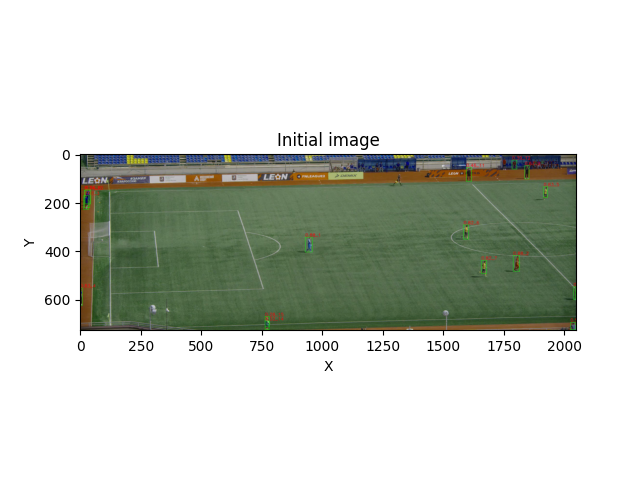
\includegraphics[width=0.8\linewidth]{figures/Initial image.png}
     \caption{Image before transformation of coordinates}
     \label{fig:before-transform}
 \end{figure}

  \begin{figure}[!ht]
     \centering
     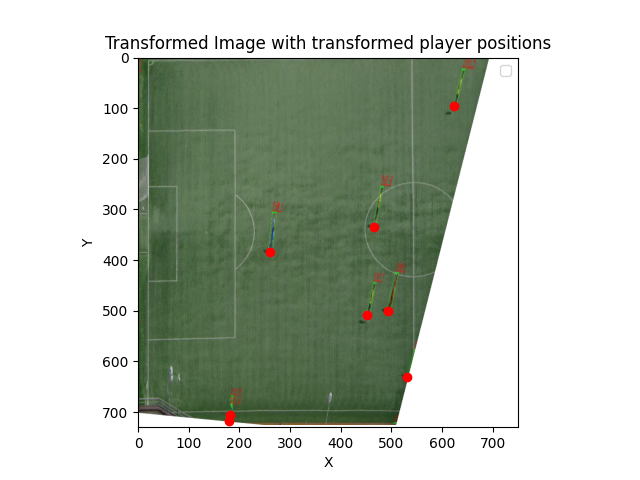
\includegraphics[width=0.8\linewidth]{figures/Transformed Image with transformed player positions.png}
     \caption{Image after transformation of coordinates}
     \label{fig:after-transform}
 \end{figure}


% Timur part
%  \section{Preprocessing}

%  \section{Algorithm Development for the Case of Static Players}
% There are many solutions for the TSP problem, but there are several key differences between them, the main one being the accuracy of the solution. Some algorithms can solve the problem of finding the minimal closed path exactly, while others do not guarantee the minimal path but are significantly faster. For this specific task, the exact solution option was chosen since the number $n$, i.e., the number of recognized objects in the frame, is small.

% Thus, according to the article~\cite{Zhang_2021}, the most optimal option was the dynamic programming method, since among the exact approaches to solving TSP, it showed the highest speed. The implemented algorithm takes one frame with recognized objects, with already transformed coordinates, the transition to which was solved in section \ref{41}, and returns a path that includes the ids of all recognized objects in the frame, in the order that minimizes the Hamiltonian closed path in the graph, whose vertices are the ids, as well as the total path length. For the next task of developing an algorithm for the case of moving players, it will probably be necessary to revise the algorithmic approach to solving the problem. Nevertheless, the dynamic programming approach can be considered successful at this stage.

\section{Camera Simulation}
\subsection{Line - Plane Intersection}
Intersection of a plane with a line:
Let $p_0$ be the camera vector, and $v_0$ be the direction vector of the light ray passing through the camera vector (center of the focal lens).

Then the parametric equation of the line can be defined as:
$$P(t) = p_0 + t \cdot v_0 \qquad \text{($P(t)$ is a point on the line)}$$

We need to find such a $t$ that $P(t)$ lies on a given plane.
Substituting this into the plane equation, we get:
$$a(P0_x + tV0_x) + b(P0_y + tV0_y) + c(P0_z + tV0_z) = d$$

Solving for $t$ ($n$ is the normal vector of the plane):
$$t = \frac{D - nP0}{n \cdot V0}$$

We are interested in $t < 0$ since positive values correspond to the wrong light direction.

\subsection{Field of View and Angle of View}
For truthful simulation of field of view and physics of long-focus cameras, work of Matvey Gancev was used (\href{https://gitlab.car.cos.ru/mgantsev/diplomagm}{Модель для панорамной камеры высокого разрешения}). As simulation of physics for camera is a complicated and time-requiring task, with the admission of Matvey Gancev, the simulation code was used. However modeling the camera movement and traversal algorithm are completed without use of intellectual property from other researchers. It is a complicated task to set the angle velocity, thus it can be estimated with a velocity on a euclidean plane. 

Field of View: The calculatePanoramicSystemFOV method calculates the angle of view (FOV) for each camera in the panoramic system and returns a list of camera angles of view for the panoramic system.

The method defines the plane vector and the coordinates and angles of the panoramic system. Then for each camera in the panoramic system, the following occurs:

\begin{enumerate}
    \item The camera coordinates and its angles of view are calculated.
    \item Vectors defining the camera's angles of view are created.
    \item Rotations are applied to the vectors of the camera and the panoramic system.
    \item The intersection point of the line (defined by the camera) with the plane (panoramic system) is calculated.
    \item The camera's angle of view and the main axis of the camera's view are calculated.
\end{enumerate}


1. Calculation of vector a:
$$
\text{vector\_a} = \begin{bmatrix}
1.0 \\
\tan\left(\frac{\text{camera\_width\_angle\_of\_view}}{2}\right) \\
-\tan\left(\frac{\text{camera\_height\_angle\_of\_view}}{2}\right)
\end{bmatrix}
$$

2. Rotation of vector $ \mathbf{a} $:
$$
\mathbf{a} = \left(\mathbf{R}_\text{ps} \cdot \mathbf{R}_\text{c}\right) \cdot \mathbf{a}
$$

Here $ \mathbf{R}_\text{ps} $ and $ \mathbf{R}_\text{c} $ are the rotation matrices for the panoramic system and the camera, respectively.

3. Re-rotation of vectors $ \mathbf{b} $, $ \mathbf{c} $, $ \mathbf{d} $, $ \mathbf{p} $:
\begin{align*}
\mathbf{b} &= \left(\mathbf{R}_\text{ps} \cdot \mathbf{R}_\text{c}\right) \cdot \mathbf{b} \\
\mathbf{c} &= \left(\mathbf{R}_\text{ps} \cdot \mathbf{R}_\text{c}\right) \cdot \mathbf{c} \\
\mathbf{d} &= \left(\mathbf{R}_\text{ps} \cdot \mathbf{R}_\text{c}\right) \cdot \mathbf{d} \\
\mathbf{p} &= \left(\mathbf{R}_\text{ps} \cdot \mathbf{R}_\text{c}\right) \cdot \mathbf{p} 
\end{align*}

Here $ \mathbf{R}_\text{ps} $ and $ \mathbf{R}_\text{c} $ are also the rotation matrices for the panoramic system and the camera.

4. Calculation of point $ \mathbf{t}_0 $:
$$
\mathbf{t}_0 = \mathbf{r}_\text{ps} + \mathbf{R}_\text{ps} \cdot \mathbf{r}_\text{c}
$$

Here $ \mathbf{r}_\text{ps} $ and $ \mathbf{r}_\text{c} $ are the coordinates of the panoramic system and the camera, respectively.

5. Definition of parameters $a_0$, $b_0$, $c_0$, $d_0$, $p_0$:

\begin{align*}
a_0 &= -\frac{\left(\mathbf{v}_\text{plane} \cdot \mathbf{v}_{\text{t}_0}\right) + D} {\left(\mathbf{v}_\text{plane} \cdot \mathbf{v}_a\right)} \\
b_0 &= -\frac{\left(\mathbf{v}_\text{plane} \cdot \mathbf{v}_{\text{t}_0}\right) + D} {\left(\mathbf{v}_\text{plane} \cdot \mathbf{v}_b\right)} \\
c_0 &= -\frac{\left(\mathbf{v}_\text{plane} \cdot \mathbf{v}_{\text{t}_0}\right) + D}{\left(\mathbf{v}_\text{plane} \cdot \mathbf{v}_c\right)} \\
d_0 &= -\frac{\left(\mathbf{v}_\text{plane} \cdot \mathbf{v}_{\text{t}_0}\right) + D}{\left(\mathbf{v}_\text{plane} \cdot \mathbf{v}_d\right)} \\
p_0 &= -\frac{\left(\mathbf{v}_\text{plane} \cdot \mathbf{v}_{\text{t}_0}\right) + D}{\left(\mathbf{v}_\text{plane} \cdot \mathbf{v}_p\right)}
\end{align*}

6. Calculation of the coordinates of the angles of view and the main axis of the camera:
\begin{align*}
\text{fov\_a} &= a_0 \cdot \mathbf{v}_a + \mathbf{v}_{\text{t}_0} \\
\text{fov\_b} &= b_0 \cdot \mathbf{v}_b + \mathbf{v}_{\text{t}_0} \\ 
\text{fov\_c} &= c_0 \cdot \mathbf{v}_c + \mathbf{v}_{\text{t}_0} \\ 
\text{fov\_d} &= d_0 \cdot \mathbf{v}_d + \mathbf{v}_{\text{t}_0} \\ 
\text{main\_axis} &= p_0 \cdot \mathbf{v}_p + \mathbf{v}_{\text{t}_0} \\
\end{align*}

These transformations are necessary to calculate the parameters of the angles of view and the main axis of the camera in the panoramic system. They perform transformations of coordinates and vectors, taking into account their initial positions and rotations relative to the coordinate system associated with the panoramic system. Then, using the found parameters, the points indicating the angles of view of each camera are determined, as well as the point representing the main axis of the camera. These steps allow us to determine the position and direction of view of each camera in the context of the panoramic system.


Angle of View: 
This method calculates the vertical angle of view of the camera. Let's consider the mathematics of this process.

Let $f$ be the focal length of the camera lens, and $H$ be the height of the camera's focal plane. We want to find the vertical angle of view $\theta_{\text{vertical}}$, which determines how many degrees vertically the camera covers.

Using the theorem of similar triangles, we understand that the vertical angle of view can be expressed as double the arctangent of the ratio of the height of the focal plane to twice the focal length:

$$
\theta_{\text{vertical}} = 2 \times \arctan \left( \frac{H}{2f} \right)
$$

Thus, we find the angle at which the image on the focal plane is visible relative to the central axis of the camera. This gives us an idea of what portion of the vertical space is covered by the image.

\subsection{Determining $\Delta$ Yaw and $\Delta$ Pitch during Movement}
To simulate the camera and the algorithm as a whole, it is important to have the ability to control the camera.
To control the camera in our study, we can send $\Delta \theta$ and $\Delta \phi$ (yaw and pitch changes) to our camera (simulated or real).

1. Central point of the field of view angles:

   Find the central point between two field of view (FOV) angles:

   Let $ P_1  $ and  $ P_2  $ be the two field of view angles of the camera, then the central point $ C  $ will be:

    $$
   C = \left( \frac{P_{1x} + P_{2x}}{2}, \frac{P_{1y} + P_{2y}}{2} \right)
    $$

2. Calculation of the angle:

   Calculate the tilt angle of the camera relative to the horizon and the vertical angle of view of the camera:

   Let $ (x_c, y_c)  $ be the coordinates of the camera, $ (x_i, y_i)  $ the initial position, and $ (x_t, y_t)  $ the target position. Also, $ h  $ is the height of the camera, and $ \theta_{\text{pitch}}  $ the vertical angle of view, $\theta_0$ the current vertical tilt angle, and $\theta_{\text{top\_aov}}$ the angle between the highest incoming light ray on the camera and the main axis of the camera ($AOV_{\text{vert}}/2$).

   First, determine the camera's yaw angle, using direction vectors from the camera to the initial and target positions:

    $$
   \Delta \theta_{\text{yaw}} = \text{atan2}(y_t - y_c, x_t - x_c) - \text{atan2}(y_i - y_c, x_i - x_c)
    $$

   Then calculate the pitch angle, which is the tilt angle of the camera relative to the horizon for:

    $$
   \theta_{\text{pitch}} = 90^\circ - \text{toDegrees}(\arctan( \frac{|(x_t-x_c, y_t-y_c) | }{h}) )
    $$

    $$
   \Delta \theta_{\text{pitch}} = \theta_{\text{pitch}} - \theta_{\text{top\_aov}} - \theta_{0}
    $$

Here, $ \text{atan2}  $ is the arc-tangent function of two arguments, $ \| \cdot \|  $ is the vector norm, and $\mod$ is the modulo operation.

\subsection{Player Detection inside of a Field of View}
It is already mentioned, that the algorithm is able to infer how close the center of FOV to the target position, but the algorithm also have a player detection module for future algorithm enhancements (for example: awaiting for the moment when player view is not obstructed by other players). 

\lstinputlisting[numbers=none]{listings/agent_in_fov.txt}


\section{Algorithm Development for the Case of Moving Players}

\begin{figure}[!ht]
    \centering
    \includesvg[width=1.0\textwidth]{figures/cam-traverse.svg}
    \caption{General Pipeline}
    \label{fig:hist_results}
\end{figure}



\subsection{Master-Route Baseline}
The basic algorithm is to pass the camera over the field in a "snake" pattern. The camera sequentially surveys each strip of the observable field, moving from the left edge of the field to the right, and then from the right edge of the field to the left. This algorithm is easily implemented once the framework from section 4.4.2 has been implemented. To cover all players, the camera can be approximated along the path when the algorithm determines that the player is close enough to its initial territory.


\pagebreak
\subsection{KNN-Greedy Algorithm}

\lstinputlisting[numbers=none]{listings/knn_greedy.txt}

In the above fragment, the main algorithm is described. 

\subsection{Probability-Density-Graphs TSP}
As a future enhancement such algorithm could be developed:

Assume we know the player graph at time t. The features of the vertices in this situation will be the coordinates of the players as well as identifiers. We train an algorithm that can predict the probabilistic distribution of each player's position over the sequence $[0,t]$ (the simplest case being a 2-dimensional Gaussian, i.e., standard normal distribution), then the goal for the camera can be set to focus on the 95\% confidence interval at time t+k, which can be calculated using the camera's angular velocity. The camera then focuses on the vertex so that the entire area is visible with sufficient confidence and zooms in on a specific player (linear interpolation of their movement can be included here). The algorithm then repeats for all players.       

\chapter{Results}

\section{Evaluation of Camera Traversal Algorithm }
\subsection{Metric and Experiment formulation}
To evaluate the algorithm, the metric chosen is time required to traverse through all players with stopping time on a player equal to $t_{stop} = 5$. Number of players $n_{players} = 22$ and $n_{iter} = 100$. An experiment will be ran $n_{iter}$ of times, and the T will be the metric for the according algorithm:
$$
T=\frac{1}{n_{iter}}\sum\limits_{i=1}^{n_{iter}} t_{i}
$$

Note that $t_{i}$ is measured in simulation ticks, with conversion formula $25  \cdot t_{i} = 1 \text{ second}$, giving FPS (frames per second) to be 25 ($FPS=25$). Also statistics like standard deviation, inter-quantile range  and histogram will be displayed for further analysis. Given the fact that PTZ cameras are often able to gather angular velocity up to 30 $^{\circ}$ per second (\href{https://www.bit-cctv.com/products/outdoor-mini-pan-tilt-positioner-head.html}{\textcolor{blue}{Source}}), given that in our case approximately 90 $^{\circ}$ of horizontal panning is enough to traverse the field and also we can not expect camera to be always on max speed, we can approximate an average speed as 18 $^{\circ}$ per second. Given such speed, it is possible to traverse the field in 5 seconds, that way yielding that on average linear speed of a camera may be roughly approximated to 20 meters per second or 0.8 meters per one frame given a FPS of 25 frames.
) 

Given such framework of evaluation, it is possible to compare quality of a baseline to the quality of the developed KNN-Greedy approach. {\color{purple}(Possibly delete a part about comparing)}

\subsection{Dataset}
To assure that experiments are representative of the real-world scenario, a  \href{https://github.com/mikecarti/hse-cam2023/tree/main/simulation}{soccer match simulation from Timur Khaibrakhmanov} was used. In the simulation, player movement is modeled with similar to real-world laws. Despite that simulation quite accurately represents football matches, it has a randomization component, that allows to create $n_{iter}=100$ diverse simulations, that represent the soccer dynamics. On those generated simulations, the algorithm is tested. Algorithm only possesses the information prior to during timestamp, thus it simulates real-world unpredictability of players' behavior.

\subsection{Result of the Experiment}
\begin{table}[h!]
\centering
\caption{Statistics of the KNN Greedy Performance for $N=100$ in frames}
\begin{tabular}{lr}
\toprule
Statistic & Frames for Complete Traversal \\
\midrule
Count     & 100.00000 \\
\textbf{Mean}      & \textbf{408.56000} \\
Standard Deviation (std) & 46.73919 \\
Minimum (min)  & 305.00000 \\
25th Percentile (25\%) & 375.75000 \\
Median (50\%)  & 412.50000 \\
75th Percentile (75\%) & 442.25000 \\
Maximum (max)  & 549.00000 \\
\bottomrule
\end{tabular}
\label{table:algorithm_stats}
\end{table}





\begin{table}[h!]
\centering
\caption{Statistics of the KNN Greedy Performance for $N=100$ in seconds}
\begin{tabular}{lr}
\toprule
Statistic & Seconds for Complete Traversal \\
\midrule
Count     & 100.00000 \\
\textbf{Mean}      & \textbf{16.3424} \\
Standard Deviation (std) & 1.8695676\\
Minimum (min)  & 12.2 \\
25th Percentile (25\%) & 15.03 \\
Median (50\%)  & 16.5 \\
75th Percentile (75\%) & 17.69 \\
Maximum (max)  & 21.96 \\
\bottomrule
\end{tabular}
\label{table:algorithm_stats}
\end{table}



\begin{figure}[!ht]
    \centering
    \includesvg[width=0.5\textwidth]{figures/experiment_n100_seconds.svg}
    \caption{Histogram of experiment in seconds}
    \label{fig:hist_results}
\end{figure}

Using the KNN Greedy algorithm yields mean of 16.3424 seconds for traversal of moving players in the case of 22 players on a 100 by 100 meters region. There are some outliers, but they have relatively low deviation from the sample mean, minimum (fastest time) is considered 12.2 seconds, and maximum is considered 21.96 seconds. Standard deviation is almost 2 second, that equates to approximately 15\% of mean, which shows robustness of the algorithm. KDE plot is similar to the bell curve of normal distribution, however left tail is much heavier, that can be interpreted as that there are a lot of surprisingly faster experiments and not quite a lot of surprisingly slow experiments (in terms of time taken to traverse all agents). One could also add that at value of 19 seconds it seems like there is some barrier that makes it hard for the simulation to take longer than this time, although it is just a hypothesis and may be due to simulation specifics.

\begin{figure}[!ht]
    \centering
    \includesvg[width=1.0\textwidth]{figures/yaw-pitch.svg}
    \caption{Yaw-Pitch Dynamics during the first simulation}
    \label{fig:yaw-pitch}
\end{figure}

Yaw pitch dynamic graph \ref{fig:yaw-pitch} represents how angle may differ through a simulation. What is worth of noting, is how pitch (tilt) changes only between 6 and 18 degrees, while yaw (panning) is spanning between 160 to 220 degrees. It gives us a hint, of how sensitive the camera FOV to the tilt compared to panning. Those 2 graphs completely describe the dynamics of a camera movement in a single simulation. Times when camera stops at a single point are almost non-visible, as it happens only for a fraction of 5 frames. There also seen the fast spikes on pitch graph, it is for now unknown what is the reasoning of such behavior, but one is certain, it may not be caused by knn-greedy algorithm.

\section{Conclusion}
In this \href{https://github.com/mikecarti/hse-cam2023}{\color{blue}study}, we endeavored to develop and assess a camera traversal algorithm tailored to the task of tracking moving players in a simulated soccer match setting. Through a systematic investigation encompassing algorithmic design, simulation, and empirical evaluation, we aimed to address the multifaceted challenges inherent in efficient field traversal and player tracking.

The foundational phase of our inquiry involved establishing rigorous coordinate systems to facilitate seamless integration between the soccer field and camera perspectives. By elucidating the transformation matrix and elucidating the interrelation between coordinate planes, we ensured a robust foundation upon which subsequent algorithmic developments could be built.

Subsequently, we delved into the intricacies of camera simulation, including the precise determination of line-plane intersections, field of view calculations, and dynamic adjustments of yaw and pitch angles during traversal. These components were pivotal in emulating realistic camera behaviors, thereby enabling the faithful reproduction of real-world scenarios within our computational framework.

The crux of our investigation lay in the algorithmic development phase, where we explored two distinct methodologies: the master-route baseline and the KNN-Greedy algorithm. The former provided a structured approach to field traversal, while the latter introduced a dynamic heuristic based on nearest-neighbor principles. Through meticulous experimentation and evaluation, we discerned significant insights into the performance and efficacy of each approach.

Our empirical findings revealed that the KNN-Greedy algorithm exhibited commendable efficiency, with an average traversal time of approximately 16.34 seconds and a standard deviation of 1.87 seconds across 100 simulation iterations. These results underscore the algorithm's robustness and efficacy in dynamically tracking moving players while navigating the soccer field.

Furthermore, our analysis extended beyond quantitative performance metrics to encompass qualitative aspects such as yaw-pitch dynamics. By visualizing the camera's orientation throughout the simulation, we gained valuable insights into its adaptability and responsiveness to evolving game scenarios, thereby elucidating avenues for further refinement and optimization.

In summation, this study represents a rigorous exploration of camera traversal algorithms in the context of tracking moving players in simulated soccer matches. By leveraging mathematical principles, computational techniques, and empirical evaluation, we have developed a sophisticated framework that bridges theoretical concepts with practical applications. Moving forward, continued research and refinement of these algorithms hold the promise of advancing the efficiency, accuracy, and versatility of camera systems in diverse sporting and surveillance domains.
%\include{6-specification}
%\section{Спецификация оборудования}

Перечень оборудования, поставленного по   Муниципальному контракту №0350300011821000371\_175478 от 04.10.2021г. на поставку серверного оборудования для подсистемы видеонаблюдения АПК «Безопасный город», серверного оборудования к существующей инфраструктуре Заказчика приведен в таблице \ref{tab:spec}.

\begin{landscape} 
\begin{center}
\begin{longtable}{|l|l|l|l|}
\caption{Спецификация оборудования поставленного по   Муниципальному контракту №0350300011821000371\_175478 от 04.10.2021г.} \label{tab:spec}  \\

\hline \multicolumn{1}{|c|}{\textbf{№}} & \multicolumn{1}{p{110pt}|}{\textbf{Наименование }} & \multicolumn{1}{p{160pt}|}{\textbf{Спецификация}}  & 
\multicolumn{1}{p{70pt}|}{\textbf{Имя и IP}} \\ \hline 
\endfirsthead

\multicolumn{4}{p{340pt}}%
{{\bfseries \tablename\ \thetable{} -- продолжение}} \\
\hline \multicolumn{1}{|c|}{\textbf{№}} & \multicolumn{1}{p{110pt}|}{\textbf{Наименование }} & \multicolumn{1}{p{160pt}|}{\textbf{Спецификация}} & 
\multicolumn{1}{p{70pt}|}{\textbf{Имя и IP}}  \\ \hline 
\endhead

\hline \multicolumn{4}{|r|}{{Продолжение на сл.странице}} \\ \hline
\endfoot

\hline \hline
\endlastfoot

1 & МВЯ -1 & Intel  i9 10900x, ddr4 32gb, sad 120gb,sfp+ 10gbit, RTX3060ti x2  & MPC01  194.255.255.0 \\\hline
2 & МВЯ -2 & Intel  i9 10900x, ddr4 32gb, sad 120gb,sfp+ 10gbit, RTX3060ti x2    & MPC02 \\\hline
3 & МХВ -1 &Intel   corei7 -9700,ОЗУ 16 Gb , 1хssd 120g+12х6тб, sfp+ 10gbit   & SS01\\\hline
4 & МХВ -2 & Intel   corei7 -9700,ОЗУ 16 Gb , 1хssd 120g+12х6тб, sfp+ 10gbit  & SS02\\\hline
5 & МХВ -3 & Intel   corei7 -9700,ОЗУ 16 Gb , 1хssd 120g+12х6тб, sfp+ 10gbit   & SS03\\\hline
6 & МХВ -4 & Intel   corei7 -9700,ОЗУ 16 Gb , 1хssd 120g+12х6тб, sfp+ 10gbit   & SS04\\\hline
7 & МХВ -5 &Intel   corei7 -9700,ОЗУ 16 Gb , 1хssd 120g+12х6тб, sfp+ 10gbit    & SS05\\\hline
8 & МХВ -6 & Intel   corei7 -9700,ОЗУ 16 Gb , 1хssd 120g+12х6тб, sfp+ 10gbit   & SS06\\\hline
9 & Коммутатор ТШ-2 & MikroTik CRS317  & MTIK317 \\\hline
10 & KVM & Aten & \\\hline
11  & Коммутатор ТШ-1  &MikroTik CRS326   & MTIK326\\\hline
12 & ИБП 10000   & IPPON 10000VA
SNMP card  & \\\hline
13  & ТШ-2   &   & \\\hline
 
\end{longtable}
\end{center}
\end{landscape}  

%\include{7-port-comm}

\backmatter %% Здесь заканчивается нумерованная часть документа и начинаются ссылки и
            %% заключение

%\chapter*{Заключение}

Разработанная  


   % Выводы 

% % Список литературы при помощи BibTeX
% Юзать так:
%
% pdflatex rpz
% bibtex rpz
% pdflatex rpz

\bibliographystyle{gost780u}
\bibliography{cam-tsp}

%%% Local Variables: 
%%% mode: latex
%%% TeX-master: "rpz"
%%% End:       % Список литературы 

%\include{98-Otzyv}

%\appendix   % Тут идут приложения

%\include{91-appendix2} 

% %\chapter*{Перечень внесенных изменений}
\Large{Лист изменений}
\small
\begin{longtable}{|p{90pt}|p{100pt}|p{260pt}|p{80pt}|}
 
\hline
\textbf{Дата} & \textbf{Автор} & \textbf{Внесенные изменения.}   \\
\hline
\endfirsthead
\multicolumn{4}{c}%
{\tablename\ \thetable\ -- \textit{Продолжение}} \\
\hline
\textbf{Дата} & \textbf{Автор} &\textbf{Внесенные изменения.}   \\
\hline
\endhead
\hline \multicolumn{4}{r}{\textit{Продолжение на следующей странице}} \\
\endfoot
\hline
\endlastfoot
  	 &   &    \\\hline
 	 &   &   \\  \hline
 	 & &    \\\hline
 	 & &    \\\hline
 	 & &    \\\hline 
 	 & &    \\\hline
 	 & &    \\\hline
 	 & &    \\\hline
 	 & &    \\\hline
 	 & &    \\\hline
 	 & &    \\\hline
 	 
\end{longtable}



\end{document}

%%% Local Variables:
%%% mode: latex
%%% TeX-master: t
%%% End:
